\newcommand{\ww}{0.49} 
\begin{figure}[H] 
    \captionsetup[subfloat]{justification=raggedright,singlelinecheck=false, position=bottom,labelformat=empty} % 
    \subfloat[Obraz O \\ ocena kontrastu k4 = 0.1088]{
       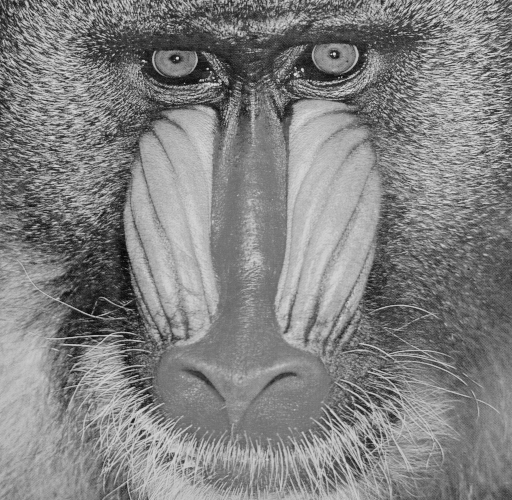
\includegraphics[width=\ww\linewidth]{../zad3/img2/I1.png}}  \hfill% 
    \subfloat[Obraz UM \\ ocena kontrastu k4 = 0.22874]{
       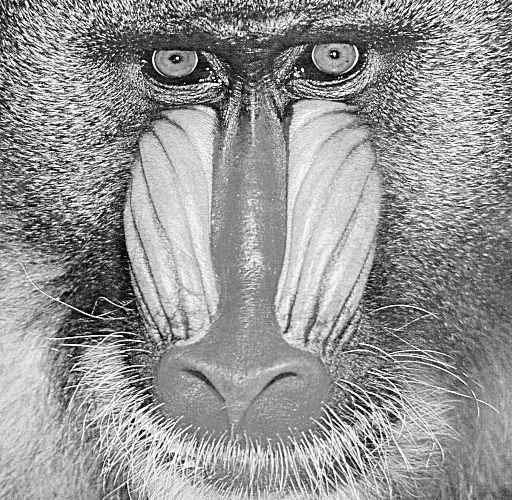
\includegraphics[width=\ww\linewidth]{../zad3/img2/I3.png}}  \\ 
    \subfloat[Metoda globalna \\ ocena kontrastu k4 = 0.24771]{
       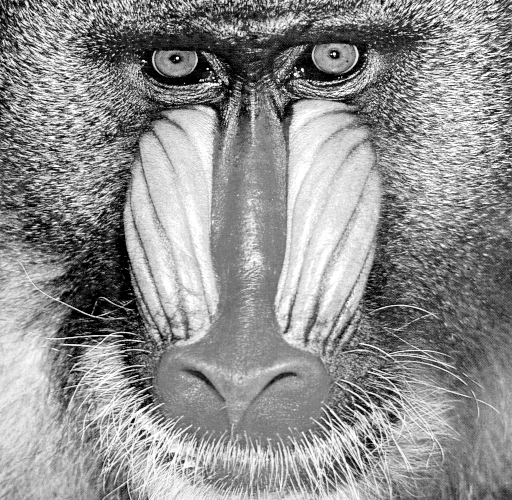
\includegraphics[width=\ww\linewidth]{../zad3/img2/I2.png}}  \hfill% 
    \subfloat[Metoda lokalna \\ ocena kontrastu k4 = 0.26946]{
       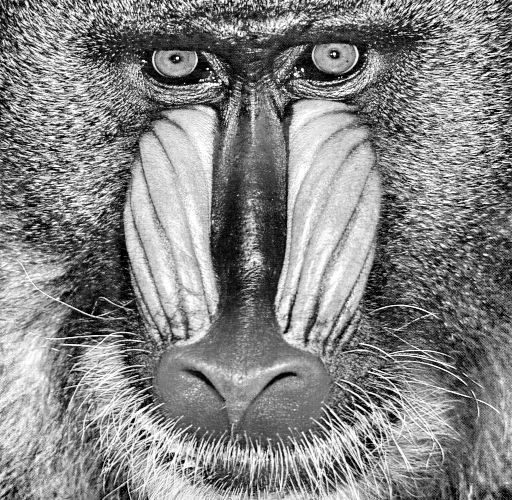
\includegraphics[width=\ww\linewidth]{../zad3/img2/I4.png}}
\caption{Porownanie wyników z różnymi metodami poprawy kontrastu}  
\label{fig:../zad3/result_2.tex} 
\end{figure} 
\let\ww\undefined 